\subsection{Automation Pyramid}
\label{subsection:automation-pyramid}
    In IIoT the two worlds of IT and OT come together, as discussed in \autoref{section:current-situation}. It doesn't come as a surprise that the OT world has its own framework for IIoT. The ``Automation Pyramid'' is one of the central frameworks in the OT world. 

    What started with the ISA-88 standard from the '90s is now closely related to the ANSI/ISA-95 standard. With the automation pyramid, we are looking at a conceptual element that strives to assert the effective and efficient distribution and connection of components in IIoT enterprises, from the shop floor to the decision-making levels and hence tries to represent all company levels. It describes the enterprise in a layered architecture where each layer can only communicate with its adjacent layers. The objective of the framework is to describe the production process from the organizational and the process perspective while providing common terminology that can be the basis for discussion \cite{umh_automation_pyramid, martinez_automation_2021}.

    \begin{figure}[htbp]
        \centering
        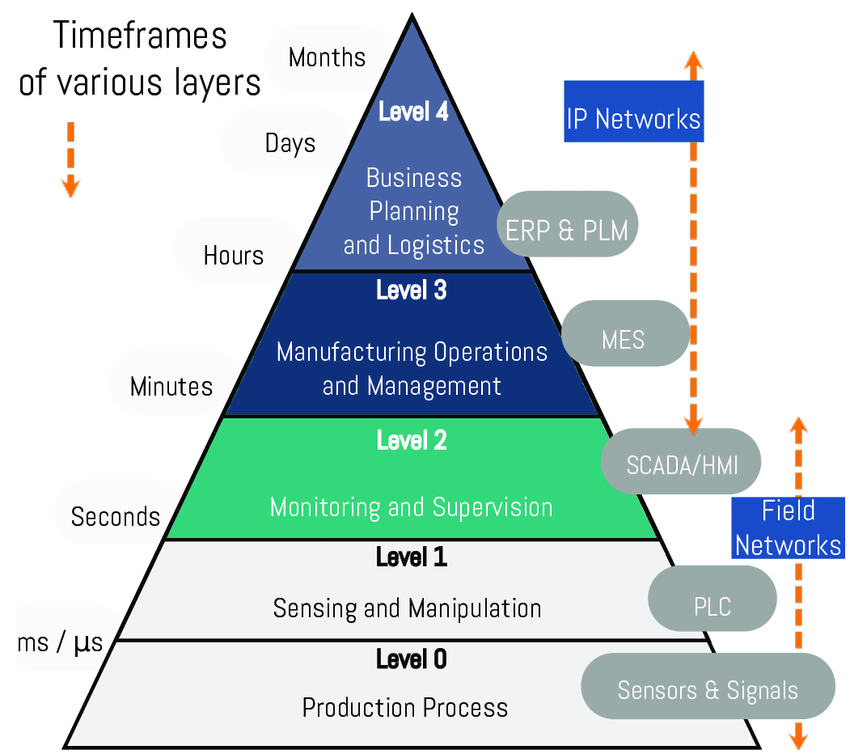
\includegraphics[width=0.6\textwidth]{img/automation-pyramid.png}
        \caption{Automation Pyramid by United Manufacturing Hub \cite{umh_automation_pyramid}}
        \label{figure:automation-pyramid}
    \end{figure}

    \noindent The layers within the automation pyramid are closely linked to the varying levels of real-time responsiveness and decision-making requirements. A shift can be seen when looking at real-time process control and monitoring at the lower layers, towards more strategic and long-term planning and analysis at the higher layers. It is also to be noted, that there is a transition from OT (bottom) to IT (top) systems in the pyramid. This structure reflects the integration of both immediate operational needs and broader organizational objectives within the automation framework which can be seen in \autoref{figure:automation-pyramid}. Starting from the bottom, the first layer represents components of the production process, which are mostly sensors or actuators. In this level (0), the actual production process is embedded which explains the high requirements regarding real-time capabilities while all subsequent levels deal with some form of automation components. The next level (1) is responsible for sensing and man\-ip\-u\-la\-tion. Typical applications within this layer deal with Programmable Logic Controllers (PLCs) that run programs that read signals from sensors or write signals to actuators. The next level (2) deals with monitoring and supervision and is the place where systems like ``Supervisory Control and Data Acquisition'' (SCADA) or ``Human Machine Interfaces'' (HMI) are located. Those might for example supervise multiple PLCs in a production process that span over a hundred meters of an assembly line where one PLC is placed every 5 meters. HMIs can e.g. be found in a control room and allow humans to visualize a control panel or to operate one or multiple machines at the same time in a remote location. The succeeding layer (3) has the responsibility of ``Manufacturing Operations and Management'', where systems like Manufacturing Execution Systems (MES) can be found. Here, management functions like generating orders are executed by the planning department. This level also houses the instruments for production and logistics, which for example includes responsibilities like decisions regarding what and when to produce. The last level (4) is called ``Business Planning and Logistics''. Here common systems for resource planning or product lifecycle management are located. This layer deals with long-term business/financial planning and is mainly responsible for organizational tasks. Inventories, billing, accounting and logistics are further things managed by this level. It is also used by many departments like finance, controlling, R\&D or sales. Depending on the system, the transition between OT and IT happens somewhere around layer 2 or 3, however the exact line to distinguish the two worlds is often blurry \cite{umh_automation_pyramid}.\newline

    As mentioned at the beginning of the chapter, the automation pyramid is a framework that mainly focuses on the OT world. It ensures that the production keeps running by combining all production-related components into autonomous layers that are not affected by casualties like IT outages. However, while this framework shines when looking at the production only, it imposes many limitations for projects dealing with large-scale IIoT systems. The main issue lies within the layered architecture. Since each component of each layer can only communicate with adjacent layers, each integration has to be built as a very specific point-to-point integration. This is very costly because many engineers with specific skill sets are required. It is also often required to use non-robust middleware to enable that communication, which can introduce many vulnerabilities into the system. The main downside of this is that it stifles innovation. Since every project comes with a high cost due to the requirement of building yet another point-to-point integration, development is slowed down immensely and thus time-to-market is heavily increased. \autoref{figure:spaghetti} shows the result of a growing system of point-to-point integrations.
    
    \begin{figure}[htbp]
        \centering
        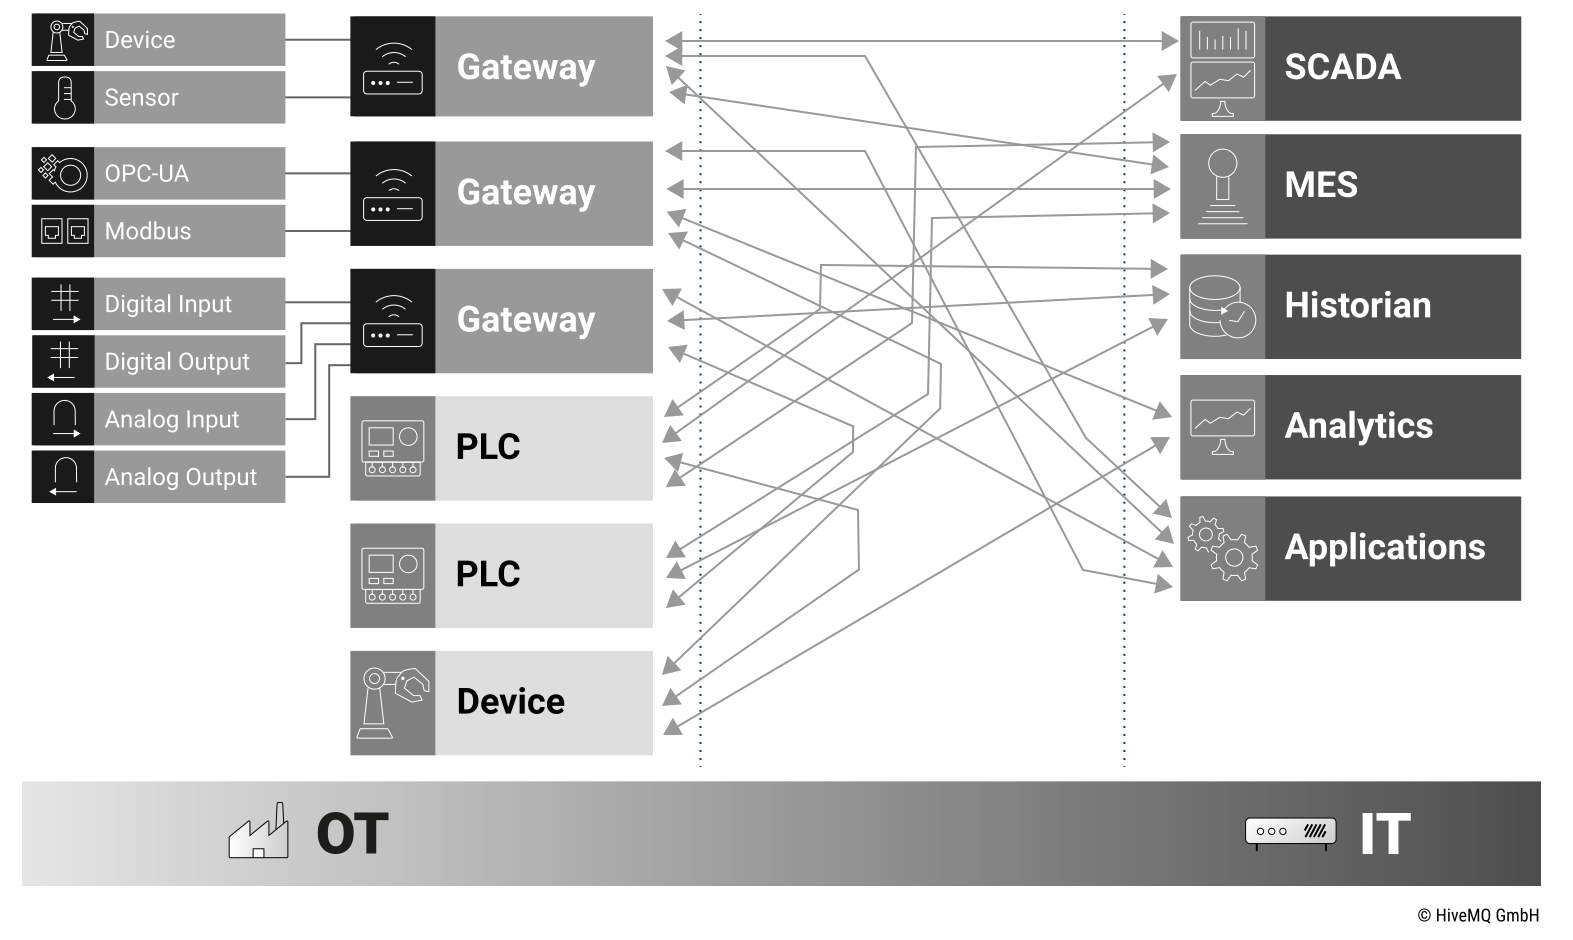
\includegraphics[width=0.9\textwidth]{img/sparkplug-01-spaghetti.png}
        \caption{Smart Manufacturing Using ISA95, MQTT Sparkplug and the Unified Namespace \cite{smart_manufacturing_using_isa95_mqtt}}
        \label{figure:spaghetti}
    \end{figure}
    
    Another issue is, that only the data that is relevant for the integration in question is sent. This means that while data is recorded at some layer, it might not be accessible on a different layer, because it was not a requirement in the integration that was built for the components. Also this results in data being siloed, which means that data recorded by one project is recorded but not available to all other projects for use due to the nature of point-to-point integrations. This is especially painful when decisions have to be made based on data of a layer, but the data is not available on the layer that is responsible for the decision yet. Lastly, the architecture leads to values based on data multiple times, since common values can't be reused by other components \cite{umh_automation_pyramid}. \newline

    Overall it is clear that the automation pyramid is not suited to serve as a reference architecture for IIoT systems. It has drawbacks that limit scalability, innovation and other key factors and clearly only fits the OT side of things. Many are aware of its shortcomings and hence move to more modern hub-and-spoke architectures. It is important to note that it brings useful components like the ISA-95 structure of levels which will be used in \autoref{section:unified-namespace} and hence serves as the basis for terminology and structure in other reference architectures.